\chapter{INTRODUCTION}
\section{HOW TO CITE}
%
The Higgs discovery is cited \cite{:2012gk}. \cite{:2012gk,PDBook} The strong interaction is given in \refeq{Eq:StrongPotential} from \refsec{Sec:QCD}.

\subsection{TABLES SUB-SECTION}
\reftab{Tab:L1Latency} is an example of a table.
%
\begin{table}
  \centering
  \caption[Level 1 Latency Table]{Table of latencies in the Level 1 systems measured in bunch-crossings of 25 ns. This is a massively parallelised operation, which is factored into the total latencies being shorter than the sum of their individual components.}
  \label{Tab:L1Latency}
  \vspace{4mm}
  \begin{tabular}{l r l}
      \toprule
      %
      ~     & \multicolumn{2}{ c }{\bf Latency}              \\
      ~     & \multicolumn{2}{ c }{\bf Contribution (BC)}    \\
      %
      \midrule
      %
      Muon Trigger                                          & \hspace{7mm} \bf 54.0         & ~    \\ 
      Calorimeter Trigger                                   & \bf 56.1                      & ~    \\
      \hspace{1cm}Cables to PPM                                        & ~                  & 20.6 \\
      \hspace{1cm}Preprocessor for CPM (e/$\gamma$, $\tau$/h)          & ~                  & 15.0 \\
      \hspace{1cm}Preprocessor for JEM (jets,\ET)                      & ~                  & 17.0 \\
      \hspace{1cm}Electron/photon hunting                              & ~                  & 14.0 \\
      \hspace{1cm}Tau/hadron hunting                                   & ~                  & 14.0 \\
      \hspace{1cm}Jet hunting                                          & ~                  & 18.0 \\
      \hspace{1cm}\MET\ calculation                                    & ~                  & 18.5 \\
      \hspace{1cm}Scalar \ET\ calculation                              & ~                  & 18.5 \\
      CTP                                                   & \bf 4.0                       & ~    \\
      TTC                                                   & \bf 3.1                       & ~    \\
      Fibres to front-end electronics                       & \bf 16.0                      & ~    \\
      Receivers for front-end electronics                   & \bf 3.0                       & ~    \\
      %
      \midrule
      %
      \bf Total Latency for L1A to reach all ROD            & \bf 82.2                      & ~    \\
      \bf Digital Pipeline Length                           & \bf 100                       & ~    \\
      %
      \bottomrule
  \end{tabular}
\end{table}

\clearpage
\subsubsection{ACRONYMS SUB-SUB-SECTION}
Acronyms are defined in {\tt acronym.tex}. Use an acronym with \verb|\ac{}|, such as the \ac{LHC}. Future use will then just show \ac{LHC}. Other uses are:
\begin{verbatim}
\acresetall
    resets all acronyms to not used. 
    Useful after the abstract to redefine all acronyms 
    in the introduction. 
\acf{label}
    written out form with acronym in parentheses, 
    irrespective of previous use 
\acs{label}
    acronym form, irrespective of previous use 
\acl{label}
    written out form without following acronym 
\acp{label}
    plural form of acronym by adding an s. 
    \acfp. \acsp, \aclp work as well. 
\end{verbatim}

\cbstart
\section{NEW CONTENT}
Use \verb|\cbstart| and \verb|\cbend| to highlight changes to the document with a red bar.
\cbend
%
%
%
%
%
\cleardoublepage
\chapter{PHYSICS}
\section{QUANTUM CHROMODYNAMICS}
\label{Sec:QCD}
%
Gluons, being themselves coloured, self interact. As a consequence, the \ac{QCD} potential between two quarks is given by 
\begin{equation}
\label{Eq:StrongPotential}
V(r) = kr - \frac{\alpha_s}{r}.
\end{equation}
Here $k$ is the spring constant from Hooke's law and $\alpha_s$ is the coupling strength of the strong interaction. Potential energy in the colour field increases linearly with separation of quarks until it is energetically favourable to pair-produce a $q\bar{q}$ pair. $\alpha_s$ is plotted in the region $2 < Q^2 < 200 \GeV$ in \reffig{Fig:qcd-running}.
%
%Note that \acs is used in the caption for the List of Figures
\begin{figure}
  \centering
  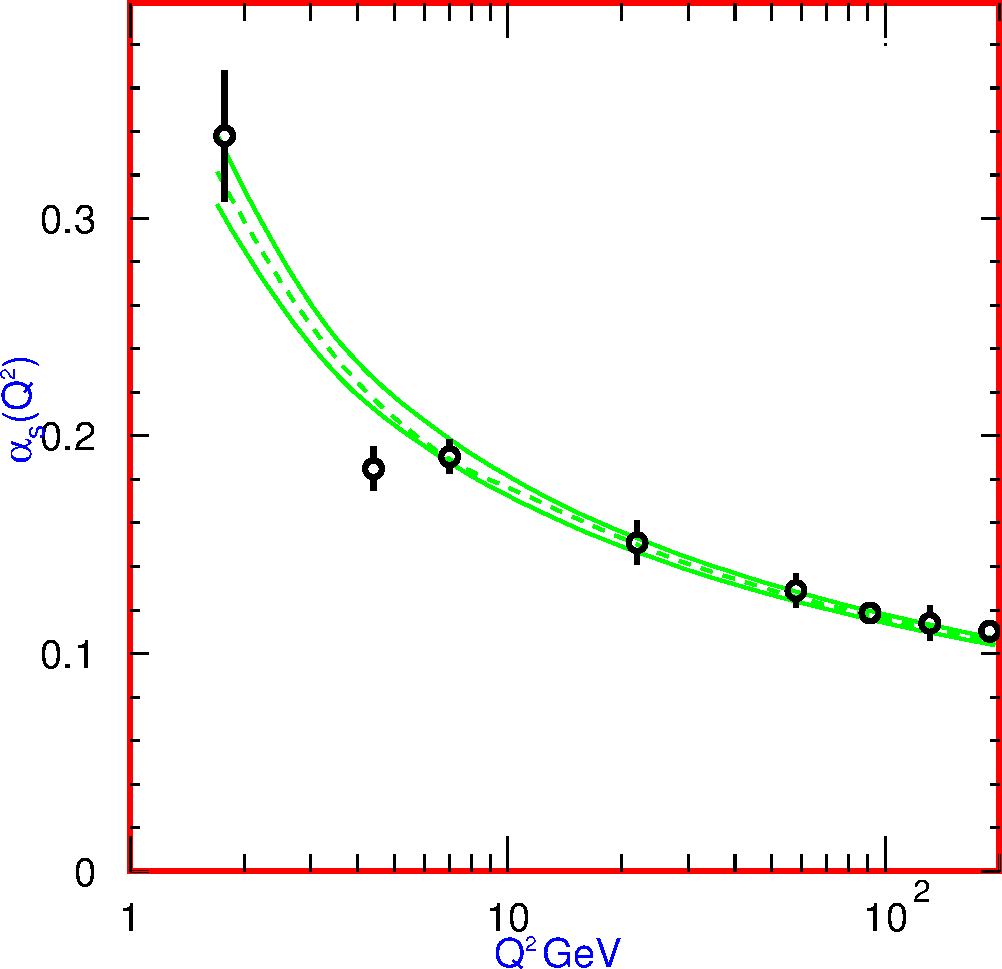
\includegraphics[width=0.75\textwidth]{fig/qcd-running}
  \caption[\acs{QCD} Running Coupling]{Strength of $\alpha_s$ as a function of energy scale. Data from various experiments are presented along with the central average and $\pm1\sigma$ limits. Taken from \cite{PDBook}.}
  \label{Fig:qcd-running}
\end{figure}

Multi-figure example in \reffig{Fig:MultiFig}
\begin{figure}
  \centering
  \subfloat[]{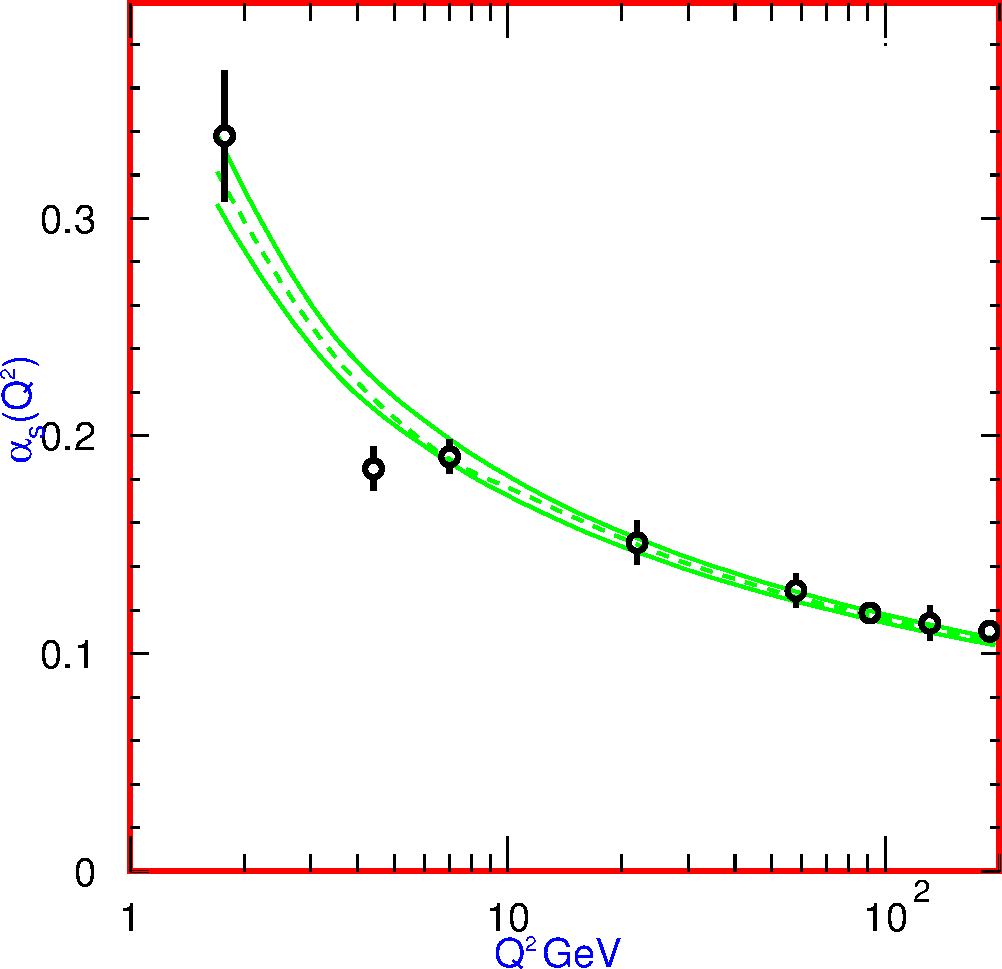
\includegraphics[width=0.48\textwidth]{fig/qcd-running}}
  \subfloat[]{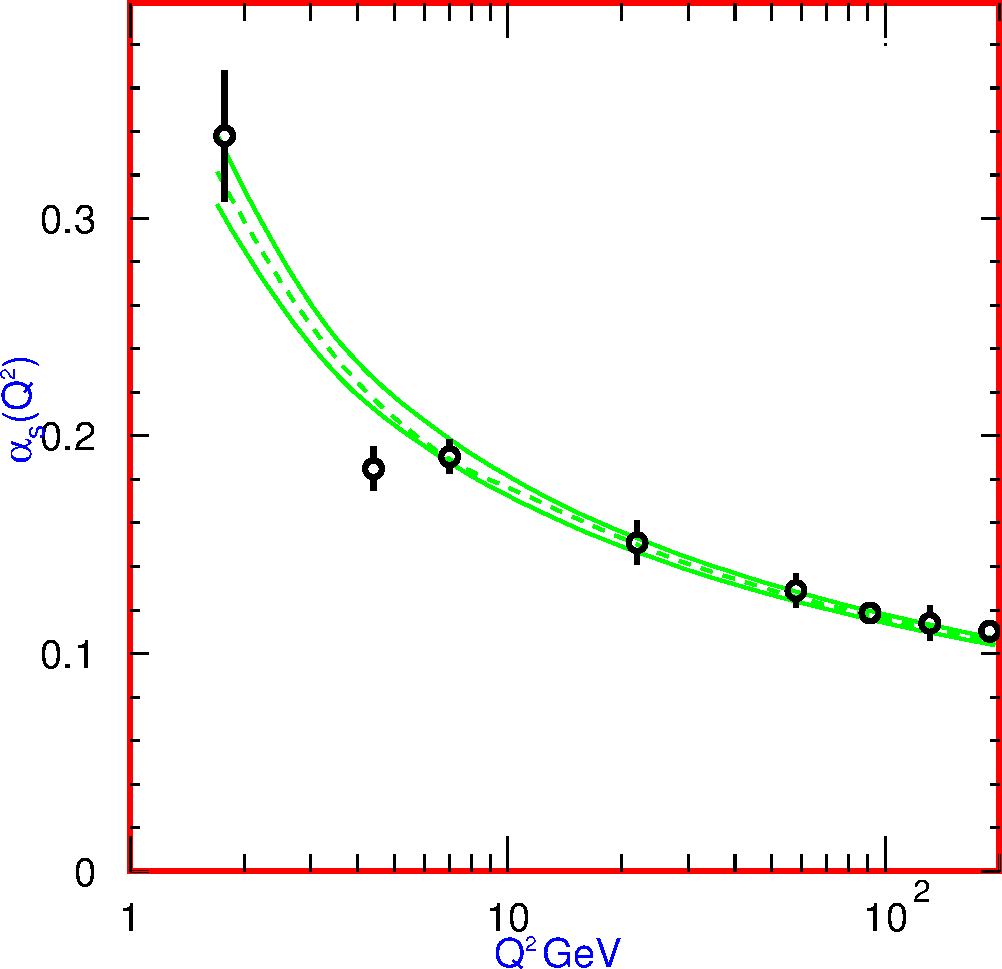
\includegraphics[width=0.48\textwidth]{fig/qcd-running}}
  \newline
  \subfloat[]{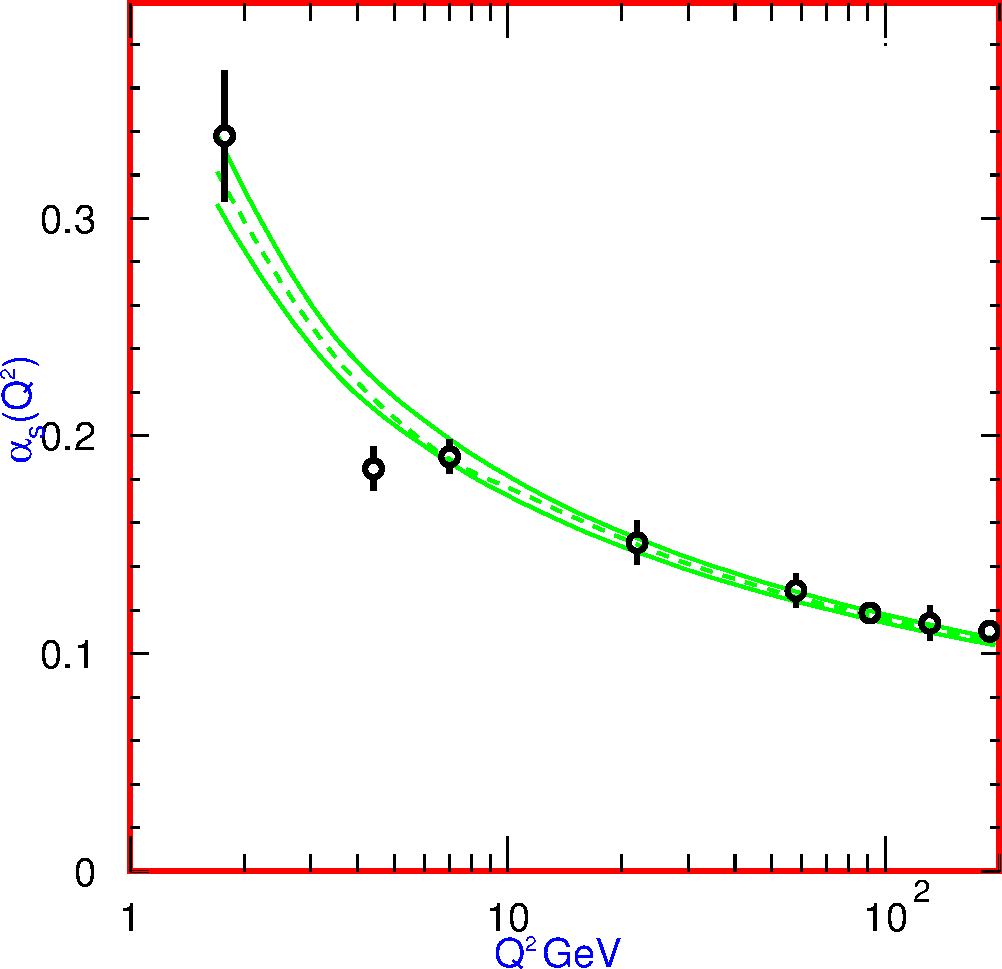
\includegraphics[width=0.48\textwidth]{fig/qcd-running}}
  \subfloat[]{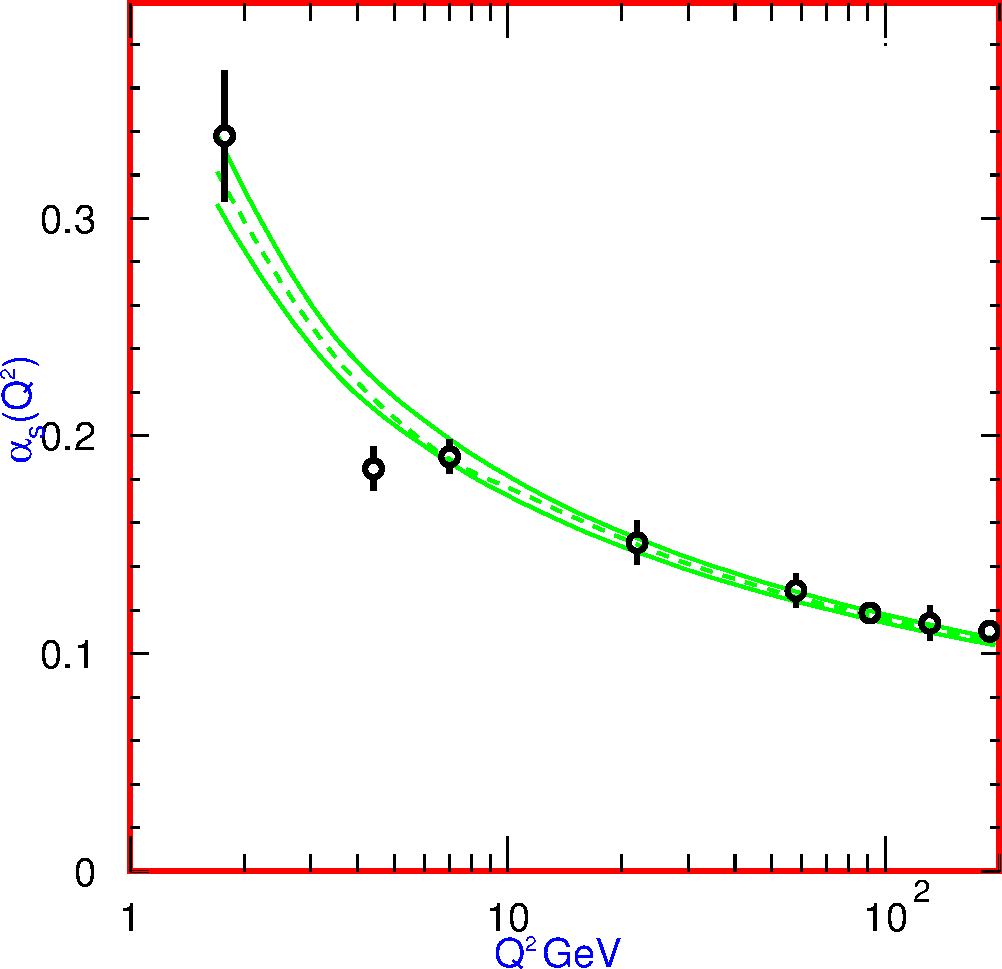
\includegraphics[width=0.48\textwidth]{fig/qcd-running}}
  \caption[Four figure example]{Example of four figures.}
  \label{Fig:MultiFig}
\end{figure}
